%----------------------------------------------------------------------------------------
%	PACKAGES AND OTHER DOCUMENT CONFIGURATIONS
%----------------------------------------------------------------------------------------

\documentclass{article}

\usepackage{fancyhdr} % Required for custom headers
\usepackage{lastpage} % Required to determine the last page for the footer
\usepackage{extramarks} % Required for headers and footers
\usepackage[usenames,dvipsnames]{color} % Required for custom colors
\usepackage{graphicx} % Required to insert images
\usepackage{listings} % Required for insertion of code
\usepackage{courier} % Required for the courier font
\usepackage{lipsum} % Used for inserting dummy 'Lorem ipsum' text into the template
\usepackage[utf8]{inputenc}
\usepackage[ngerman]{babel}

% Margins
\topmargin=-0.45in
\evensidemargin=0in
\oddsidemargin=0in
\textwidth=6.5in
\textheight=9.0in
\headsep=0.25in

\linespread{1.1} % Line spacing

% Set up the header and footer
\pagestyle{fancy}
%\lhead{\hmwkAuthorName} % Top left header
\chead{\hmwkClass\ : \hmwkTitle} % Top center head
\rhead{\firstxmark} % Top right header
\lfoot{\lastxmark} % Bottom left footer
\cfoot{} % Bottom center footer
\rfoot{Page\ \thepage\ of\ \protect\pageref{LastPage}} % Bottom right footer
\renewcommand\headrulewidth{0.4pt} % Size of the header rule
\renewcommand\footrulewidth{0.4pt} % Size of the footer rule

\setlength\parindent{0pt} % Removes all indentation from paragraphs

%----------------------------------------------------------------------------------------
%	CODE INCLUSION CONFIGURATION
%----------------------------------------------------------------------------------------

\definecolor{MyDarkGreen}{rgb}{0.0,0.4,0.0} % This is the color used for comments
\lstloadlanguages{Perl} % Load Perl syntax for listings, for a list of other languages supported see: ftp://ftp.tex.ac.uk/tex-archive/macros/latex/contrib/listings/listings.pdf
\lstset{language=Perl, % Use Perl in this example
        frame=single, % Single frame around code
        basicstyle=\small\ttfamily, % Use small true type font
        keywordstyle=[1]\color{Blue}\bf, % Perl functions bold and blue
        keywordstyle=[2]\color{Purple}, % Perl function arguments purple
        keywordstyle=[3]\color{Blue}\underbar, % Custom functions underlined and blue
        identifierstyle=, % Nothing special about identifiers                                         
        commentstyle=\usefont{T1}{pcr}{m}{sl}\color{MyDarkGreen}\small, % Comments small dark green courier font
        stringstyle=\color{Purple}, % Strings are purple
        showstringspaces=false, % Don't put marks in string spaces
        tabsize=5, % 5 spaces per tab
        %
        % Put standard Perl functions not included in the default language here
        morekeywords={rand},
        %
        % Put Perl function parameters here
        morekeywords=[2]{on, off, interp},
        %
        % Put user defined functions here
        morekeywords=[3]{test},
       	%
        morecomment=[l][\color{Blue}]{...}, % Line continuation (...) like blue comment
        numbers=left, % Line numbers on left
        firstnumber=1, % Line numbers start with line 1
        numberstyle=\tiny\color{Blue}, % Line numbers are blue and small
        stepnumber=5 % Line numbers go in steps of 5
}

% Creates a new command to include a perl script, the first parameter is the filename of the script (without .pl), the second parameter is the caption
\newcommand{\perlscript}[2]{
\begin{itemize}
\item[]\lstinputlisting[caption=#2,label=#1]{#1.pl}
\end{itemize}
}

%----------------------------------------------------------------------------------------
%	DOCUMENT STRUCTURE COMMANDS
%	Skip this unless you know what you're doing
%----------------------------------------------------------------------------------------

% Header and footer for when a page split occurs within a problem environment
\newcommand{\enterProblemHeader}[1]{
%\nobreak\extramarks{#1}{#1 continued on next page\ldots}\nobreak
%\nobreak\extramarks{#1 (continued)}{#1 continued on next page\ldots}\nobreak
}

% Header and footer for when a page split occurs between problem environments
\newcommand{\exitProblemHeader}[1]{
%\nobreak\extramarks{#1 (continued)}{#1 continued on next page\ldots}\nobreak
%\nobreak\extramarks{#1}{}\nobreak
}

\setcounter{secnumdepth}{0} % Removes default section numbers
\newcounter{homeworkProblemCounter} % Creates a counter to keep track of the number of problems

\newcommand{\homeworkProblemName}{}
\newenvironment{homeworkProblem}[1][Problem \arabic{homeworkProblemCounter}]{ % Makes a new environment called homeworkProblem which takes 1 argument (custom name) but the default is "Problem #"
\stepcounter{homeworkProblemCounter} % Increase counter for number of problems
\renewcommand{\homeworkProblemName}{#1} % Assign \homeworkProblemName the name of the problem
\section{\homeworkProblemName} % Make a section in the document with the custom problem count
%\enterProblemHeader{\homeworkProblemName} % Header and footer within the environment
}{
%\exitProblemHeader{\homeworkProblemName} % Header and footer after the environment
}

\newcommand{\problemAnswer}[1]{ % Defines the problem answer command with the content as the only argument
\noindent\framebox[\columnwidth][c]{\begin{minipage}{0.98\columnwidth}#1\end{minipage}} % Makes the box around the problem answer and puts the content inside
}

\newcommand{\homeworkSectionName}{}
\newenvironment{homeworkSection}[1]{ % New environment for sections within homework problems, takes 1 argument - the name of the section
\renewcommand{\homeworkSectionName}{#1} % Assign \homeworkSectionName to the name of the section from the environment argument
\subsection{\homeworkSectionName} % Make a subsection with the custom name of the subsection
%\enterProblemHeader{\homeworkProblemName\ [\homeworkSectionName]} % Header and footer within the environment
}{
%\enterProblemHeader{\homeworkProblemName} % Header and footer after the environment
}

%----------------------------------------------------------------------------------------
%	NAME AND CLASS SECTION
%----------------------------------------------------------------------------------------

\newcommand{\hmwkTitle}{Übung\ \#4} % Assignment title
\newcommand{\hmwkDueDate}{Donnerstag,\ 27.\ November\ 2014} % Due date
\newcommand{\hmwkClass}{GPU Computing} % Course/class
\newcommand{\hmwkClassTime}{} % Class/lecture time
\newcommand{\hmwkClassInstructor}{} % Teacher/lecturer
\newcommand{\hmwkAuthorName}{Günther Schindler, Alexander Schapp, Klaus Naumann} % Your name

%----------------------------------------------------------------------------------------
%	TITLE PAGE
%----------------------------------------------------------------------------------------

\title{
\vspace{2in}
\textmd{\textbf{\hmwkClass:\ \hmwkTitle}}\\
\normalsize\vspace{0.1in}\small{Abgabe\ am\ \hmwkDueDate}\\
\vspace{0.1in}\large{\textit{\hmwkClassTime}}
\vspace{3in}
}

\author{\textbf{\hmwkAuthorName}}
\date{} % Insert date here if you want it to appear below your name

%----------------------------------------------------------------------------------------

\begin{document}

\maketitle

%----------------------------------------------------------------------------------------
%	TABLE OF CONTENTS
%----------------------------------------------------------------------------------------

%\setcounter{tocdepth}{1} % Uncomment this line if you don't want subsections listed in the ToC
\newpage
\tableofcontents
\newpage

%----------------------------------------------------------------------------------------
%	Reading
%----------------------------------------------------------------------------------------

\begin{homeworkProblem}[Reading]
\subsection{NVIDIA TESLA : A UNIFIED GRAPHICS AND COMPUTING ARCHITECTURE}
The authors Erik Lindholm, John Nickolls, Stuart Oberman and John Montrym discuss in 
'NVIDIA TESLA : A UNIFIED GRAPHICS AND COMPUTING ARCHITECTURE' the requirements that
drove the unified graphics and parallel computing processor architecture, describe the 
Tesla architecture, and how it is enabling widespread deployment of parallel computing 
and graphics applications. Main reasons for developing the new architecture was to
enable flexible, programmable graphics and high performance computing. The primary
goal of this contribution is to introduce the new architecture and their capabilities.

Key insight of the new architecture is the new processor architecture called
single-instruction, multiple-thread (SIMT), which is similar to single-instruction,
multiple-data (SIMD) design, but applies one instruction to multiple independent 
threads in parallel. Due to the new architecture, each streaming multiprocessor 
is able to execute 24 warps (32 parallel threads). With that a streaming multiprocessor
manages and executes up to 768 concurrent threads in hardware with zero scheduling
overhead.

This contribution is more a promotional guide then an objective article about the NVIDIA 
Tesla architecture. However, the introduced architecture and their capabilities is 
ground-breaking for the high performance computing. Although the SIMT model needs
capable programmers and fixed calculation problems to attain success in computing.

\subsection{Debunking the 100X GPU vs. CPU Myth}
In this paper the author wants to verify wether the use of a GPU on throuphut computing with large amount of data-level parallislm results in a substanable speedup of 10X up to 100X compared to the use of a CPU.
 To acheive that he compares the perfomance of the Nvidia GTX280 GPU and a Intel Core i7-960 CPU on different workloads.
  He recognizes a speed-up that is heavily depending of the  current workload, but in average the GPU shows a speed-up of only about 2.5X, so markebly lower than the prediction of other papers.

His first reason for this is that you have to make sure you compare your probably optimized GPU code with an also opimized CPU-version.
Thereby also the different possibilities of opimising on CPUs (multithreading & cache blocking) and GPUs (minimizing global synchronization & using local shared buffers) are discussed.
His second reason is that you also use compareble hardware components, so not compare e.g. a high performance
GPU to a mobile CPU. 
The violation of both could leed to the predicted optimistic speed-ups. 

Over all the argumentation of the author, why the predicted speed-up  of 10-1000X is very much lower, is quite reasonable, but as a reader it is hard to believe that all the other papers are neglegting his rules of 'compare equal to equal' in such a hefty way, since this should actually be clear as a rule.
\end{homeworkProblem}

%----------------------------------------------------------------------------------------
%	Shared Memory Analysis - Basics
%----------------------------------------------------------------------------------------

\begin{homeworkProblem}[Shared Memory Analysis - Basics]

\end{homeworkProblem}
%----------------------------------------------------------------------------------------
%	Shared Memory Analysis - Conflicts
%----------------------------------------------------------------------------------------
\begin{homeworkProblem}[Shared Memory Analysis - Conflicts]
Folgender Kernel lädt Daten von Shared Memory in das Thread-lokale Register. Jeder
Thread operiert genau auf einem Element vom Typ float. Die Zeit, bzw. die Taktzyklen, 
werden mit der clock64() funktion ermittelt. Für die Messungen werden 32 Threads per 
Block verwendet. Dies entspricht der Anzahl an Threads die in einer Gruppe 
zusammengefasst, gleichzeitig ausgeführt werden und dient somit am bestern der Analyse
der Bank Conflicts. Da multiple Thread-Blöcke auch ihre eigenen Shared Memory Bereiche
hervorrufen wird hier auch nur mit einem Thread-Block analysiert.
\begin{lstlisting}{c}
__global__ void 
bankConflictsRead(float * outFloat, int iStride, unsigned long long *ullTime)
{
  /* Static size of shared memory */
  __shared__ float s_memoryA[2024];
  /* Variable in register */
  float r_var;
  /* Start measure clock cycles */
  unsigned long long startTime = clock64();
  /* Access data from shared memory to register */
  r_var = s_memoryA[threadIdx.x*iStride];
  /* End measure clock cycles */
  *ullTime = clock64() - startTime;
  /* Conditionally assign register var, so it wont get optimized */
  if(threadIdx.x == 0) outFloat[0] = r_var;
}
int main()
{
  bankConflictsRead <<< 1, 32 >>> (outFloat, optStride, d_ullTime);
}
\end{lstlisting}
Shared Memory ist in verschiedene Bänke unterteilt. Jede dieser Bänke kann nur einen
Zugriff auf einmal verarbeiten. Wird innerhalb einer Warp Ausführung mehrmals auf eine 
Bank zugegriffen, wird der Zugriff serialisiert und benötigt somit mehr Zeit.

Folgender Plot zeigt die benötigte Clock Anzahl in Abhänigkeit von dem verwendeten
Stride. 
\begin{center}
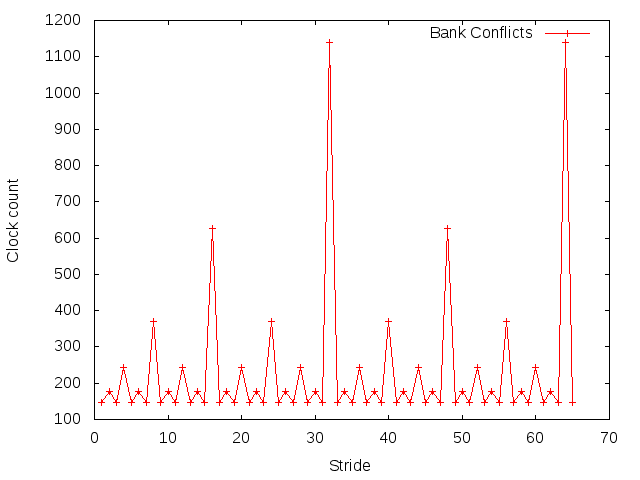
\includegraphics[width=0.8\columnwidth]{conflicts.png}
\end{center}

Der Plot verdeutlicht, dass der Zugriff nur dann konfliktfrei abläuft, wenn der Stride
keinen gemeinsamen Teiler mit der Bankanzahl besitzt. So müssen bei einem Stride von 
2, 6, 10, 14, etc. zwei Zugriffe serialisert werden. Bei einem Stride 4, 12, 20, etc.
müssen vier Zugriffe serialisiert werden. Dieser Trend setzt sich bis zu einem Stride
von 32 fort, wobei alle 32 Zugriffe serialisert werden müssen.

Übersteigt der Stride die Anzahl von 32 fängt der Trend wieder von vorne an. Dies 
bedeutet, dass ein ganzes vielfaches der Bankanzahl erreicht ist und somit Shared
Memory in 32 Bänke unterteilt ist.
\end{homeworkProblem}

%----------------------------------------------------------------------------------------
%	Matrix Multiply – CPU sequential version
%----------------------------------------------------------------------------------------

\begin{homeworkProblem}[Matrix Multiply – CPU sequential version]

\end{homeworkProblem}
\pagebreak
\end{document}